\section{topic a}
\label{sec:related_work:jigsaw_puzzles}
\addcontentsline{tocheb}{section}{\protect\numberline{\secnumforhebrewtoc}{נושא א}}

To be continued.


\section{topic b}
\label{sec:related_work:relaxation_labeling}
\addcontentsline{tocheb}{section}{\protect\numberline{\secnumforhebrewtoc}{נושא ב}}

To be continued.

\subsection{sub topic b.1}
\label{subsec:formulation_as_rl:rationale:type_2}
\addcontentsline{tocheb}{subsection}{\protect\numberline{\subsecnumforhebrewtoc}{תת נושא ב1}}

To be continued.

\begin{figure}[H]
    \centering
    
    \begin{subfigure}[b]{0.3\textwidth}
        \begin{tikzpicture}
            \node[anchor=south west, inner sep=0] at (0,0) {
\includegraphics[width=\textwidth]{content/related_work/images/2x2_puzzle_grid.png}};
            \draw[step=0.5\textwidth] (0,0) grid (\textwidth,\textwidth);
            \node[font=\large] at (0.25\textwidth,0.75\textwidth) {(1,1)};
            \node[font=\large] at (0.75\textwidth,0.75\textwidth) {(1,2)};
            \node[font=\large] at (0.25\textwidth,0.25\textwidth) {(2,1)};
            \node[font=\large] at (0.75\textwidth,0.25\textwidth) {(2,2)};
        \end{tikzpicture}
        \caption{}
        \label{fig:type_1_goal_and_labeling:dimensions}
    \end{subfigure}
    \hfill
    \begin{subfigure}[b]{0.3\textwidth}
        \begin{tikzpicture}
            \node[anchor=south west, inner sep=0] at (0,0) {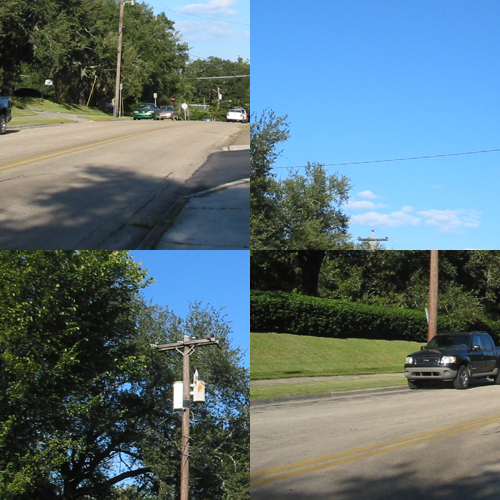
\includegraphics[width=\textwidth]{content/related_work/images/2x2puzzle_type_1.png}};
            \draw[step=0.5\textwidth] (0,0) grid (\textwidth,\textwidth);
            \node[font=\large, color=red] at (0.25\textwidth,0.75\textwidth) {Piece 1};
            \node[font=\large, color=red] at (0.75\textwidth,0.75\textwidth) {Piece 2};
            \node[font=\large, color=red] at (0.25\textwidth,0.25\textwidth) {Piece 3};
            \node[font=\large, color=red] at (0.75\textwidth,0.25\textwidth) {Piece 4};
        \end{tikzpicture}
        \caption{}
        \label{fig:type_1_goal_and_labeling:pieces}
    \end{subfigure}
    \hfill
    \begin{subfigure}[b]{0.3\textwidth}
        \begin{tikzpicture}
            \node[anchor=south west, inner sep=0] at (0,0) {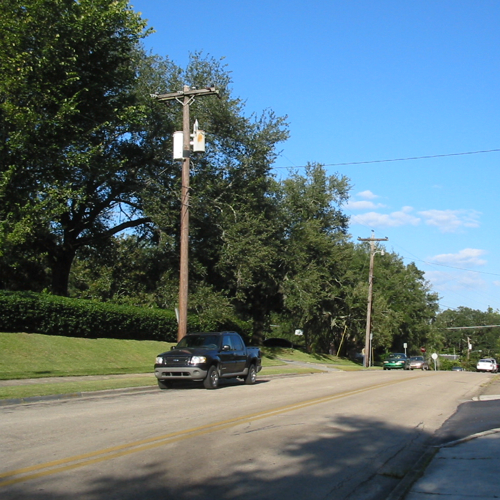
\includegraphics[width=\textwidth]{content/related_work/images/2x2puzzle_solution.png}};
            \draw[step=0.5\textwidth] (0,0) grid (\textwidth,\textwidth);
            
            \node[font=\large, color=red] at (0.25\textwidth,0.75\textwidth) {Piece 3};
            
            \node[font=\large, color=red] at (0.75\textwidth,0.75\textwidth) {Piece 2};
            
            \node[font=\large, color=red] at (0.25\textwidth,0.25\textwidth) {Piece 4};
            
            \node[font=\large, color=red] at (0.75\textwidth,0.25\textwidth) {Piece 1};
        \end{tikzpicture}
        \caption{}
        \label{fig:type_1_goal_and_labeling:solution}
    \end{subfigure}
    \vfill
    \begin{subfigure}[b]{1\textwidth}
        \centering
    
        \begin{tikzpicture}
        \def\scaletitles{0.88}
        \def\minimumEntrySize{0.95cm}

        \matrix[matrix of nodes,
        nodes={draw, align=center, minimum size=\minimumEntrySize},
        row 1/.style={nodes={draw=none, gray, font=\footnotesize, scale=\scaletitles}},
        column 1/.style={nodes={draw=none, gray, font=\footnotesize,
        scale=\scaletitles}}]
        {
            \node{}; & 
            \node{(1,1)}; & 
            \node{(1,2)}; & 
            \node{(2,1)}; &
            \node{(2,2)};\\
            %----------%
            \node{Piece 1}; &
            \node{0}; & \node{0}; & \node{0}; & \node[text=blue]{1};\\
            %----------%
            \node{Piece 2}; &
            \node{0}; & \node[text=blue]{1}; & \node{0}; & \node{0};\\
            %----------%
            \node{Piece 3}; & 
            \node[text=blue]{1}; & \node{0}; & \node{0}; & \node{0};\\
            %----------%
            \node{Piece 4}; & 
            \node{0}; & \node{0}; & \node[text=blue]{1}; & \node{0};\\
        };
        \end{tikzpicture}
        \caption{}
        \label{fig:type_1_goal_and_labeling:labeling}
    \end{subfigure} 
    \caption[fig A - Example for fig]{Some example}
    \label{fig:type_1_goal_and_labeling}
\end{figure}


\begin{table}[H]
\centering
\begin{tabular}{ |c|c|c|c|c|c| } 
 \hline
 \multicolumn{1}{|c|}{Puzzle Type} & Direct & Neighbor & Perfect & Occupied & Feasible \\ 
 \hline
    Type 1 & {0\%} & {0.1\%} & 0 & {1\%} & 0 \\ 
 \hline
    Type 2 & {0.001\%} & {0.1\%} & 0 & {1.2\%} & 0 \\ 
  \hline
\end{tabular}
\caption[Table A -  Example for table]{Some example}
\label{table:plain_rl_results}
\end{table}